\documentclass{article}
\usepackage[utf8]{inputenc}
\usepackage{color}
\usepackage{hyperref}
\usepackage{minted}
\usepackage{graphicx}
\usepackage{listings}
\usepackage{fancyhdr}
\title{Quadrocopter Raspberry Pi 2016\\Universtität Tübingen\\Marcel Früh}


\lhead{QuadroCopter RaspberryPi}
\pagestyle{fancy}

%%%%
%CODE ANPASSEN SENSORDATEN
%APP


%%%


\begin{document}
\maketitle
\begin{enumerate}
\item[] \textbf{Vorwort:}

\item[] Im Studiengang Informatik der Universität wird jedes Sommersemester das Teamprojekt durchgeführt, was für die Studierenden Pflicht ist. Es wurden eine vielzahl verschiedener Projekte angeboten, darunter auch die Arbeit an der Software des Quadrocopters.\\
Das Ziel des Projektes war die Anpassung der Low Level Treiber um die Sensor Daten in Echtzeit auszulesen, diese an eine Datenbank zu schicken, aus welcher dann die GUI die Daten abruft und in einem Oszilloskop anzeigt. Desweiteren wurde auf der Arbeit des letzen Semesters aufgebaut und eine Funktion erstellt, welche die Kontrolle der ,nun über die Programmiersprache C ansteuerbaren, Motoren von außerhalb zulässt. Außerdem wurde ein Testfall erstellt, welcher das Testen der Funktionalität der GUI sehr leicht ermöglicht.\\

Unser Team bestand am Anfang des Projektes aus den drei Gruppen: Datenbank, Embedded System und GUI. Die Teams wurden im Laufe des Projektes erweitert. Es kamen Team App und Team Project Management dazu.\\
Wir trafen uns in der Regel alle 2 Wochen um unsere Erfolge, sowie auch Misserfolge, zu präsentieren und das weitere Fortfahren des Projektes zu besprechen.\\

An dieser Stelle möchte ich mich recht herzlich bei Chris Mönch, Oliver Breuning und Jürgen Schmidt für die ausgezeichnete Dokumentation des Quellcodes und der Programmierung des Raspberry Pis bedanken.
\end{enumerate}

\newpage

\tableofcontents

\vspace{2cm}
\begin{center} 
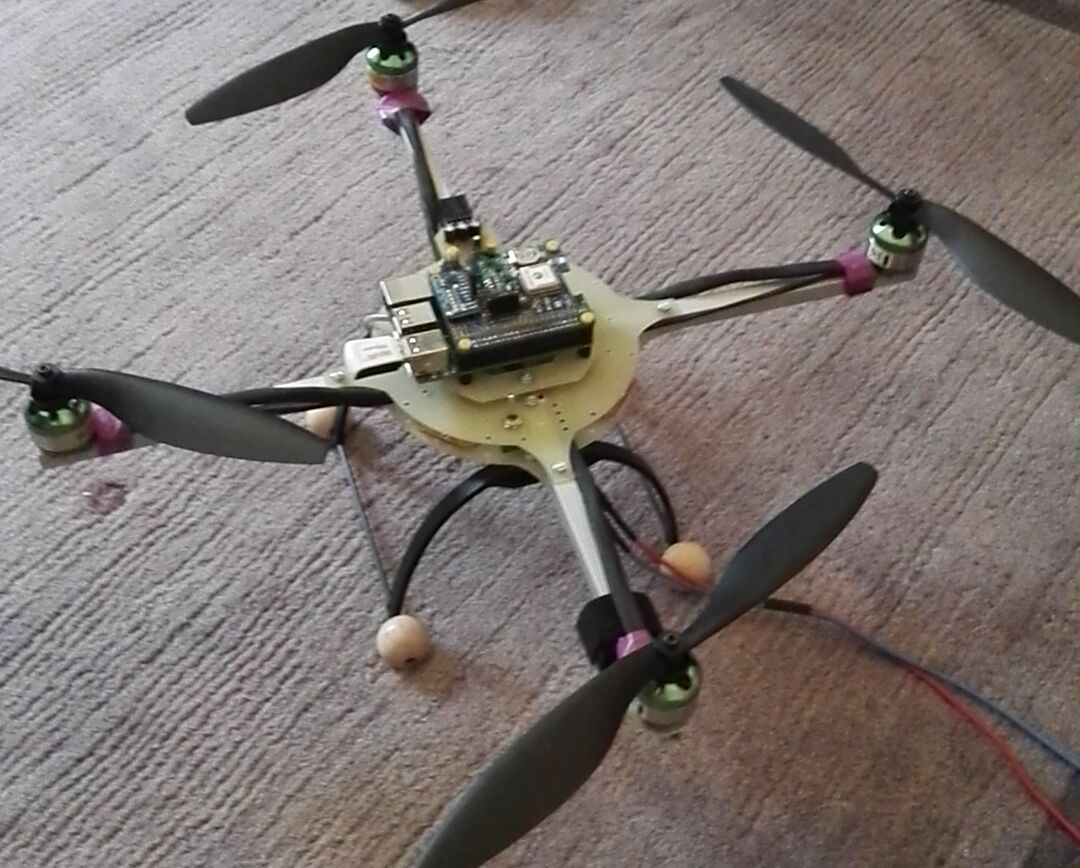
\includegraphics[width=0.9\textwidth]{graphics/signal.jpeg}
\end{center}


\newpage
\section{Grundlagen}
\subsection{Entwicklungsumgebung}

\begin{enumerate}
\item[]Das schreiben von Funktionen für den Quadrocopter ist am Anfang nicht direkt ohne weiteres möglich. Da jegliche Software über den angebrachten Raspberry Pi ausgeführt wird, müssen einige Sachen beachtet werden.\\

Einen der wichtigsten Faktoren möchte ich direkt vorneweg nehmen: Das Kompilieren der Software findet nicht auf dem Raspberry Pi direkt statt, sondern über \textcolor{red}{\textbf{Cross Compiling}}\ auf dem Entwicklungs PC. Dies wird in einem eigenen Abschnitt nähers erläutert.\\

Nun werde ich im Folgenden die notwendigen Schritte beschreiben, um Ihnen einen sofortigen und unkomplizierten Einstieg zu ermöglichen.\\

\end{enumerate}
\subsection{Betriebssystem}
Auf Grund des oben genannten Cross Compilings ist Windows als Betriebssystem nicht geeignet. Sie können selbstverständlich eine Virtual Machine nutzen, auf welcher Linux läuft. Die Anleitung zur Einrichtung dieser Machine können sie der Anleitung QuadrocopterSetup entnehmen.\\
Ich selbst habe keine Virtual Box verwendet, sondern unter Ubuntu 14.04 gearbeitet, es kann aber jede Linux Umgebung verwendet werden.\\

\subsection{IDE}
\begin{enumerate}

\item[]Ich habe eclipse als IDE verwendet, da es Cross Compiling unterstützt und Remote Debugging erlaubt.\\
Die Installation von Eclipse funktioniert wie folgt:\\
\item Downloaden Sie Eclipse IDE for C/C++ Developers unter  \footnote{Stand 12.8.2016}\\ 

\begin{center}

\url{http://www.eclipse.org/downloads/eclipse-packages/}\\ 

\end{center}

Beachten Sie dabei, dass es eine 32 und eine 64 Bit Version gibt!\\

\item Entpacken des Downloads in OPT (ermöglicht globale Nutzung)
\begin{minted}{bash}
cd /opt/ && sudo tar -zxvf ~/Downloads/eclipse-*.tar.gz
\end{minted}

\item ShortCut erstellen
\begin{minted}{bash}
sudo gedit /usr/share/applications/eclipse.desktop
\end{minted}

In diese Datei schreiben Sie folgendes:\\

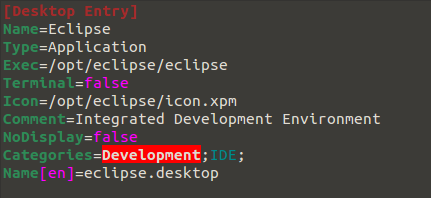
\includegraphics[width=0.8\textwidth]{graphics/eclipse.png}

Nun können sie eclipse über die Suche finden und starten!\\
\end{enumerate}

\subsection{Toolchain for Cross Compiling}
\begin{enumerate}
\item[] Zuerst: Was ist Cross Compiling?\\
Unter Cross Compiling versteht man, das Kompilieren von ausführbaren Dateien auf einer Plattform für eine andere Plattform.
Genau dies geschieht bei diesem Projekt. Wir kompilieren auf unserem Rechner eine ausführbare Datei für den Raspberry PI. Sie können gerne versuchen die Datei einmal auszuführen. Die Konsole wird ihnen einen Fehler werfen.\\

Zurück zur Toolchain:\\

\item Installieren Sie git, falls noch nicht getan.
\begin{minted}{bash}
sudo apt-get install build-essential git
\end{minted}

\item Nun wechseln Sie in das Quadrocopter Verzeichnis. Dort befindet sich der Ordner helikopter-tools. Gehen Sie in diesen Ordner und klonen sie die Toolchain. Bei mir hatte Der Ordner den Namen Quadrocopter-RaspberryPi. 

\begin{minted}{bash}
cd Quadrocopter-RaspberryPi/helikopter-tools
git clone https://github.com/raspberrypi/tools
\end{minted}

\item Falls durch den Klon ein Überordner angelegt wird gehen Sie in diesen und Kopieren alle vorhandenen Ordner in helikopter-tools und löschen Sie den Überordner. Gehen Sie nun in den Ordner arm-bcm2708. Dort befinden sich 4 Ordner. Führen Sie nun folgende Befehle aus:\\

\begin{minted}{bash}
cd ~
gedit .bashrc
export PATH=$PATH:$HOME/cd Quadrocopter-RaspberryPi/helikopter-tools/arm-bcm2708
/gcc-linaro-arm-linux-gnueabihf-raspbian-x64/bin
\end{minted}
Falls Sie eine 32 Bit Plattform benutzen nehmen Sie den Ordner ohne x64\\

\item Nun wird nur noch die Pfad Variable geupdated und Sie sind bereit loszulegen:\\

\begin{minted}{bash}
arm-linux-gnueabihf-gcc -v
\end{minted}

Sie sollten nun dieses Bild sehen:\\
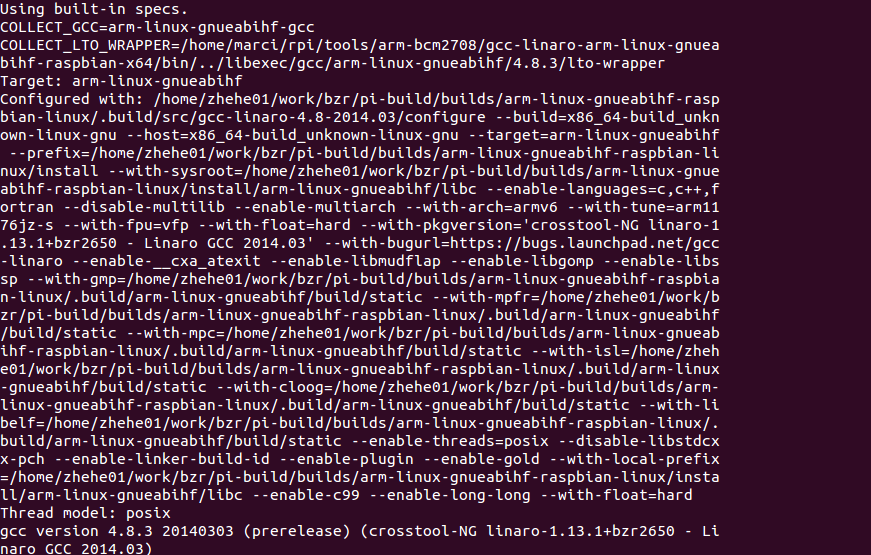
\includegraphics[width=0.9\textwidth]{graphics/arm.png}
\end{enumerate}

Herzlichen Glückwunsch! Sie sind nun bereit loszulegen.

\subsection{CMake}

\begin{enumerate}
\item[] Um den Code zu kompilieren haben wir CMake verwendet. Der Vorteil von Cmake ist, dass nur die CMakeList.txt benötigt wird und alle anderen Makefiles generisch von Cmake erstellt werden.\\

\item Installation:

\begin{minted}{bash}
sudo apt-get install cmake
\end{minted}

\item Um Cmake nun zu nutzen erstellen wir uns einen build Ordner im Quadrocopter Verzeichnis und starten dort cmake mit dem Oberverzeichnis in dem sich CMakeList.txt befindet.

\begin{minted}{bash}
mkdir Quadrocopter-RaspberryPi/build
cd  Quadrocopter-RaspberryPi/build
cmake ..
\end{minted}
\item Jegliche Änderungen am Kompilierungsvorgang werden nun in der CMakeList.txt durchgeführt. Insbesondere steht in dieser Datei auch der Befehl, welcher den Code via scp auf den Raspberry Pi schickt.
Sie müssen also nur make im build Verzeichnis aufrufen, und der Code wird kompiliert + die ausführbare Datei auf den Pi gespielt.\\
Falls die IP Adresse angepasst werden muss, lassen Sie einfach gedit nach der Zeile scp Helikopter suchen. Dort werden Sie die die IP Adresse finden.\\

\end{enumerate}

\subsection{Raspberry PI}
\begin{enumerate}
\item[] Um das Programm nun auszuführen muss zuerst eine Verbindung zu dem Raspberry PI aufgebaut werden. Dazu sind folgende Schritte notwendig. Es wird unterschieden, ob eine Verbindung via WLAN oder via Ethernet aufgebaut wird.
\begin{center}
\underline{Ethernet}:\\
\end{center}

\item Es wird die Config: /etc/network/interfaces aufgerufen:
\begin{minted}{bash}
sudo gedit /etc/network/interfaces

\end{minted}
Dort werden nun folgende Informationen eingetragen:\\

\begin{center}
\begin{tabular}{|c|}
\hline
allow-auto eth1\\
iface eth1 inet static\\
address 192.168.22.160\\
netmask 255.255.255.0\\
gateway 192.168.22.9\\
\hline
\end{tabular}


\end{center}

Die Adresse kann dabei selbstverständlich angepasst werden.

\item Nun verbinden sie ihren Rechner via Ethernet mit dem Pi. Sie können jetzt eine Verbindung via ssh herstellen.\\
Dazu rufen sie wieder das Terminal auf und geben folgendes ein:\\

\newpage
\begin{minted}{bash}
ssh pi@192.168.22.161
\end{minted}
Das Passwort ist zum jetzigen Zeitpunkt: \emph{raspberry}\\

\item Um unnötige Schreibarbeit zu sparen wurde die IP Adresse in der /etc/hosts mit einem ALIAS versehen. Dazu führen Sie folgende Befehle aus:
\begin{minted}{bash}
sudo gedit /etc/hosts
\end{minted}
Dort wird folgendes eingetragen:\\
\begin{center}

\begin{tabular}{|c|}
\hline
192.168.22.161 helikopter\\
\hline
\end{tabular}

\end{center}

Nun können Sie die Verbindung deutlich angenehmer herstellen:
\begin{minted}{bash}
ssh pi@helikopter
\end{minted}

Sie sind nun mit dem Raspberry PI verbunden und können über das Terminal Befehle eingeben.

\item Ihr Programm führen sie mit:
\begin{minted}{bash}
sudo ./HELIKOPTER
\end{minted}
aus.\\

\begin{center}
\underline{WLAN}
\end{center}
\end{enumerate}
\begin{enumerate}


\item[]Um eine Verbindung über WLAN herzustellen verbinden Sie sich mit der bereitgestellten FritzBox. Der Raspberry wird dies automatisch machen, sobald der WIPI Stick eingesteckt worden ist. Die automatische Verbindung des Raspberry Pis wird folgendermaßen eingerichtet:\\

\item
\begin{minted}{bash}
sudo nano /etc/network/interfaces
\end{minted}
Dort wird folgendes hinzugefügt, falls nicht vorhanden:\\

\begin{center}

\begin{tabular}{|c|}
\hline
allow-hotplug wlan0\\
iface wlan0 inet static\\
address 192.168.178.161\\
netmask 255.255.255.0\\
gateway 192.168.178.1\\
\hline
\end{tabular}
\end{center}

\item In die WPA Supplicant.conf wird folgendes eingetragen:\\

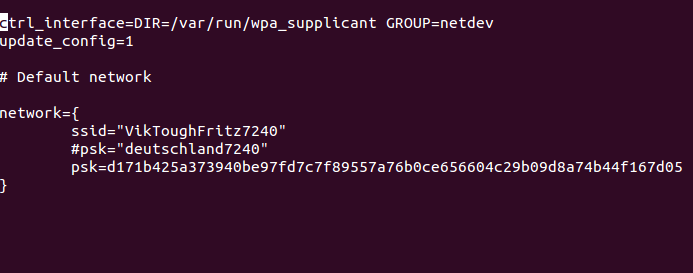
\includegraphics[width=1.2\textwidth]{graphics/wpa.png}\\
Statt dem Hashkey können Sie auch das Passwort in Klartext (hier auskommentiert) eingeben. Oder Sie generieren sich einen neuen Hashkey.\\

\item Als letztes wird der WPA Supplicant noch in den Autostart gelegt, damit die Verbindung bei jedem Starten hergestellt wird.

\begin{minted}{bash}
sudo nano /etc/rc.local
\end{minted}
Dort wird folgendes eingefügt, falls nicht vorhanden:\\


\includegraphics[width=1.1\textwidth]{graphics/wpa2.png}

Nun kann die Verbindung auch über WLAN aufgebaut werden:\\
Dazu wird wieder auf ihrem PC im Terminal folgender Befehl ausgeführt:
\begin{minted}{bash}
ssh pi@192.168.178.161
\end{minted}
Dafür können Sie sich natürlich auch wieder einen ALIAS anlegen wenn Sie möchten.\\

\item[] \underline{WICHTIG}:\\
Um das Ansteuern der Rotoren zu ermöglichen muss das braun blaue Kabel an den SCL Pin und das braun-rote Kabel an den SDA Pin der kleinen Platine angeschlossen werden!

\end{enumerate}

\newpage


\section{Hauptteil}
\subsection{UDP Sockets}
\begin{enumerate}
\item[] Da sich bei meinen Aufgaben sehr viel um Senden und Empfangen via UDP gedreht hat, ist hier der Aufbau einer Funktion, die die Aussage \emph{"Hallo Welt"} an die angegebene IP Adresse sendet.\\


\begin{minted}{c}
#include <stdio.h>
#include <stdlib.h>
#include <string.h>
#include <unistd.h>
#include <sys/types.h>
#include <sys/socket.h>
#include <netinet/in.h>

int main(){
int clientSocket;
struct sockaddr_in serverAddress;
socklen_t addressSize;

char toSend[10] = "Hallo Welt\n";

clientSocket = socket(PF_INET, SOCK_DGRAM, IPPROTO_UDP);

serverAddress.sin_family = PF_INET;
serverAddress.sin_port = htons("5000");	// Port
serverAddress.sin_addr.s_addr = inet_addr("192.168.22.160");	// IP Adresse

memset(serverAddress.sin_zero, '\0',sizeof(serverAddress.sin_zero));
addressSize = sizeof(serverAddress);

sendto(clientSocket, toSend, sizeof(toSend), 0,
		(struct sockaddr *) &serverAddress, addressSize);

}
\end{minted}

\end{enumerate}
\newpage
\subsection{Testen der GUI}
\begin{enumerate}
\item[]Es wurde ein Testfall geschrieben, welcher über UDP eine zufällige Zahl im Intervall $\lbrack 0,149 \rbrack$ schickt. Um die Gui nicht zu überlasten wurde in jedem Durchgang eine Sekunde Pause gemacht. Die UDP Sockets sind die selben wie oben.
\begin{minted}{c}
while (1) {
    sleep(1);
    int random = rand() % 150;
    char randomToSend[3];
    sprintf(randomToSend, "%i\n", random);
    sendto(clientSocket, randomToSend, sizeof(randomToSend), 0,
			(struct sockaddr *) &serverAddress, addressSize);
	printf("And send again....\n");
}
\end{minted}

Eine sehr wichtige Funktion beim Senden von Daten ist:
\begin{minted}{c}
int sprintf ( char * str, const char * format, ... );
\end{minted}

Diese Funktion weist nämlich unserem zu sendenden char Array einen formatierten Inhalt zu.
Im obigen Beispiel weisen wir unserem char randomToSend mittels dem Spezifizierer i den Wert random zu. Der Spezifizierer i gibt an, dass random ein Integer ist. Nun steht in randomToSend der randomisierte Wert und kann mittels sendto gesendet werden.\\

Die wichtigsten Spezifizierer, welche benötigt wurden sind:\\

\begin{tabular}{|c|c|}
\hline
Spez. & Bedeutung\\
\hline
c & Character\\
s & String (von Charactern)\\
f & float\\
i & integer\\
u & unsigned integer\\
\hline
\end{tabular}

Bei dem Versenden der Sensordaten hatte diese Funktion eine besonders große Bedeutung.\\

\newpage

\subsection{Versenden der Sensordaten}
\item[]Eine Hauptaufgabe des Projekts war das Versenden der Sensordaten an das Datenbank Team, welche die Daten entgegennahm, sie verarbeitet hat und dann in die Datenbank eingefügt hat. Damit wir unabhängig voneinander arbeiten konnten, mussten wir uns zuerst ein Protokoll erstellen,welche Daten versendet werden sollen und vor allem, wie sie gesendet werden, damit das Datenbank Team die Daten zuordnen kann.
Somit wurde in die Testsammlung in der main.c ein "Test" finalsending aufgenommen.

Das Protokoll sieht folgendermaßen aus:\\

\begin{tabular}{|c|c|}
\hline
Sensor Daten & Darstellung gemäß Protokoll\\
\hline
Zeit in Sekunden & TimS12345678.9\\
Zeit in Millisekunden & TimM12345678.9\\
\hline
Beschleunigung x-Achse & AccX12345678.9\\
Beschleunigung y-Achse & AccY12345678.9\\
Beschleunigung z-Achse & AccZ12345678.9\\
\hline
Magnet Wert x-Achse & MagX12345678.9\\
Magnet Wert y-Achse & MagY12345678.9\\
Magnet Wert z-Achse & MagZ12345678.9\\
\hline
Gyroskop yaw & GyrY12345678.9\\
Gyroskop pitch & GyrP12345678.9\\
Gyroskop roll & GyrR12345678.9\\
\hline
Temperatur & Temp12345678.9\\
Druck & Pres12345678.9\\
\hline
Motor1 & Mot112345678.9\\
Motor2 & Mot212345678.9\\
Motor3 & Mot312345678.9\\
Motor4 & Mot412345678.9\\
\hline

\end{tabular}\\


Das Versenden der Sensordaten verursachte einige Zeit Probleme, da die Daten zwar richtig abgesendet wurden, am Ziel selbst kam allerdings nur Nonsense an.

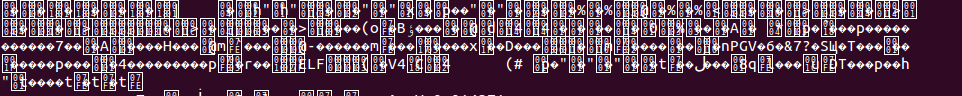
\includegraphics[width=1.3\textwidth]{graphics/kry.png}\\
\newpage
Das Problem lag an 2 Ursachen:
\item Die erste Ursache war, dass die Daten doppelt gesendet wurden. Der Befehl  l\_udpSocket\_i32 hat die Daten ebenfalls an die Remote Ip Adresse gesendet. Dieser Befehl wurde irrtümmlicherweise in den Code mit eingebunden, obwohl eigentlich mittels der sendto Funktion gesendet werden soll.
\item Die zweite Ursache lag an falschen Größen. Dadurch, dass die chars fast alle die Größe 16 haben, wurden auch immer 16 Bytes gesendet. Dies war bei vielen Werten deutlich zu groß. Mittels sprintf konnte dieses Problem nun behoben werden. Wie oben beschrieben liefert sprintf einen int Wert als Rückgabe. Dieser entspricht der tatsächlichen Größe der Sensordaten.  

Die Aufgabe wurde nun folgendermaßen umgesetzt:\\

\begin{minted}{c}
//Preparation for Sensor Calls
            halImu_orientationValues l_imuMeasurements_st;
            g_halImu_initImuSensors_bl();

            printf("Start Sending \n");
            //Sensor Data

            //Sensor Data
            while (1) {

                g_halImu_triggerImuReading_bl();
                g_halImu_triggerBaroReading_bl();
                g_halImu_triggerGyroReading_bl();
                g_halImu_triggerAccReading_bl();

                //Get Sensor Data and Timestamp

                l_imuMeasurements_st = g_halImu_getImuValues_str();

                long ms; // Milliseconds
                struct timespec spec;
                time_t res;
                res = time(NULL);
                clock_gettime(CLOCK_REALTIME, &spec);
                ms = round(spec.tv_nsec / 1.0e6); // nano -> mili

                //Call SensorData an save them in floats

                float ax = l_imuMeasurements_st.acc.x_f64;
                float ay = l_imuMeasurements_st.acc.y_f64;
                float az = l_imuMeasurements_st.acc.z_f64;

                float mx = l_imuMeasurements_st.mag.x_f64;
                float my = l_imuMeasurements_st.mag.y_f64;
                float mz = l_imuMeasurements_st.mag.z_f64;

                float y = l_imuMeasurements_st.gyro.yaw_f64;
                float p = l_imuMeasurements_st.gyro.pitch_f64;
                float r = l_imuMeasurements_st.gyro.roll_f64;

                float t = l_imuMeasurements_st.temperature_f64;
                float pr = l_imuMeasurements_st.pressure_f64;

                //No Motor running : ZERO
                int mot1 = 0;
                int mot2 = 0;
                int mot3 = 0;
                int mot4 = 0;

                clocks = sprintf(tis, "TimS%u\n", res);
                clockms = sprintf(tims, "TimM%u\n", ms);
                int sizeC = clocks+clockms;
                accx = sprintf(imu_x, "AccX%f\n", ax);
                int sizeAccX = sizeC+accx;
                accy = sprintf(imu_y, "AccY%f\n", ay);
                int sizeAccY = sizeAccX+accy;
                accz = sprintf(imu_z, "AccZ%f\n", az);
                int sizeAccZ = sizeAccY +accz;

                magx = sprintf(mag_x, "MagX%f\n", mx);
                int sizemagX = sizeAccZ +magx;

                magy = sprintf(mag_y, "MagY%f\n", my);
                int sizemagY = sizemagX +magy;

                magz = sprintf(mag_z, "MagZ%f\n", mz);
                int sizemagZ = sizemagY +magz;


                gy = sprintf(g_y, "GyrY%f\n", y);
                int sizeGy = sizemagZ+gy;
                gp = sprintf(g_p, "GyrP%f\n", p);
                int sizeGp = sizeGy+gp;

                gr = sprintf(g_r, "GyrR%f\n", r);
                int sizeGr = sizeGp+gr;


                temp = sprintf(tmp, "Temp%f\n", t);
                int sizeTemp = sizeGr + temp;
                press = sprintf(prs, "Pres%f\n", pr);
                int sizePress = sizeTemp + press;
                m1 = sprintf(Motor1, "Mot1%u\n", mot1);
                int sizeM1 = sizePress + m1;
                m2 = sprintf(Motor2, "Mot2%u\n", mot2);
                int sizeM2 = sizeM1+ m2;
                m3 = sprintf(Motor3, "Mot3%u\n", mot3);
                int sizeM3 = sizeM2+m3;
                m4 = sprintf(Motor4, "Mot4%u\n", mot4);
                int sizeM4 = sizeM3+m4;



                memcpy(buffer, tis, clocks);
                memcpy(buffer + clocks, tims, clockms);
                memcpy(buffer + sizeC, imu_x, accx);
                memcpy(buffer + sizeAccX, imu_y, accy);
                memcpy(buffer + sizeAccY, imu_z, accz);
                memcpy(buffer + sizeAccZ, mag_x, magx);
                memcpy(buffer + sizemagX, mag_y, magy);
                memcpy(buffer + sizemagY, mag_z, magz);
                memcpy(buffer + sizemagZ, g_y, gy);
                memcpy(buffer + sizeGy, g_p, gp);
                memcpy(buffer + sizeGp, g_r, gr);
                memcpy(buffer + sizeGr, tmp, temp);
                memcpy(buffer + sizeTemp, prs, press);
                memcpy(buffer + sizePress, Motor1, m1);
                memcpy(buffer + sizeM1, Motor2, m2);
                memcpy(buffer + sizeM2, Motor3, m3);
                memcpy(buffer + sizeM3, Motor4, m4);

                sendto(send, buffer, sizeof(buffer), 0,
                        (struct sockaddr *) &sendAddr, addressSize);

                printf(tis, '\n');
                printf(tims, '\n');
                printf(imu_x, '\n');
                printf(imu_x, '\n');
                printf(imu_z, '\n');
                printf(mag_x, '\n');
                printf(mag_y, '\n');
                printf(mag_z, '\n');
                printf(g_y, '\n');
                printf(g_p, '\n');
                printf(g_r, '\n');
                printf(tmp, '\n');
                printf(prs, '\n');
                printf(Motor1, '\n');
                printf(Motor2, '\n');
                printf(Motor3, '\n');
                printf(Motor4, '\n');


                sleep(1);
            }
        }
\end{minted}

Damit die kompletten Daten in einem einzelnen Sendto gesendet werden können, wurde ein ausreichend großer Buffer mittels memcpy befüllt und dieser Buffer dann versendet. Wichtig zu erwähnen ist, dass wir memcpy die richtige aufaddierte Größe übergeben, damit an der korrekten Stelle des Buffers eingefügt wird.\\
Die Daten werden nun auch beim Empfänger korrekt und richtig formatiert angezeigt!\\
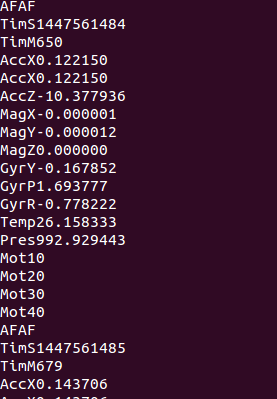
\includegraphics[height=7.3cm]{graphics/sensor.png}\\

Im Bild kann man sehr gut die ankommenden Sensordaten und deren "Verpackung" erkennen.Die Datenbank muss jeweils bloß die ersten 4 Buchstaben abschneiden und prüfen, zu welchen Daten diese gehören.\\
\\

Diese Daten werden auch in den anderen Testfällen nun gesendet. Somit können die Daten nun auch während die Motoren laufen gesendet werden und man kann die Änderungen sehr gut auf dem Oszilloskop beobachten.\\

\end{enumerate}

\subsection{Rotorentest}
\begin{enumerate}

\item[] Es wurde ein Testfall pleasefly geschrieben, der zuerst 2 Eingaben erwartet, nämlich einen MAX-PWM Wert und eine Stepsize.\\
In diesem Testfall wird nun der PWM Wert der Motoren auf den eingegebnen Maximalwert erhöht. Je nach Stepsize Wert geschieht dies langsam oder sehr schnell. Wird der maximale Wert erreicht, wird der PWM Wert wieder um die Stepsize verringert. Dieser Vorgang wird so oft  wiederholt bis manuell abgebrochen wird.\\

Da die ganze Zeit die Sensordaten mitgeschickt werden, kann man sehr schön sehen, wie sich die Werte bei wechselnden PWM Werten verändern. Der Code wurde folgendermaßen implementiert:
\begin{minted}{c}
printf("Beschleunigungstest \n");

char pwm[3];
char step[3];

char BLCtrlADRExecuteOrder[DEFMotorsCount];
char sendBuffer[1];
unsigned int pwmValue;
int STEPSIZE;
int MAXPWMVALUE = 0;

printf("Eingabe maximaler PWM Wert, 2 Ziffern < 70 \n");
scanf("%s", pwm);
MAXPWMVALUE = atoi(pwm);
printf("Eingabe Stepsize, 1 Ziffer, < 10\n");
scanf("%s", step);
STEPSIZE = atoi(step);

GetBLCtrlADRExecuteOrder(&BLCtrlADRExecuteOrder[0]);

while(1){
	while(pwmValue < MAXPWMVALUE){}

		//Sensordaten werden wie oben versendet

		//Sending Values over I2c

		sendBuffer[0] = pwmValue;

		g_lldI2c_WriteI2c_bl(BLCtrlADRExecuteOrder[0],
			&sendBuffer[0], 1);
		g_lldI2c_WriteI2c_bl(BLCtrlADRExecuteOrder[1],
			&sendBuffer[0], 1);
		g_lldI2c_WriteI2c_bl(BLCtrlADRExecuteOrder[2],
			&sendBuffer[0], 1);
		g_lldI2c_WriteI2c_bl(BLCtrlADRExecuteOrder[3],
			&sendBuffer[0], 1);
		usleep(100000);

		pwmValue = pwmValue + STEPSIZE;

}

	while (pwmValue > 5) {
		//Sensordaten werden wie oben versendet
    
		//Sending Values over I2c

		sendBuffer[0] = pwmValue;

		g_lldI2c_WriteI2c_bl(BLCtrlADRExecuteOrder[0],
			&sendBuffer[0], 1);
		g_lldI2c_WriteI2c_bl(BLCtrlADRExecuteOrder[1],
			&sendBuffer[0], 1);
		g_lldI2c_WriteI2c_bl(BLCtrlADRExecuteOrder[2],
			&sendBuffer[0], 1);
		g_lldI2c_WriteI2c_bl(BLCtrlADRExecuteOrder[3],
			&sendBuffer[0], 1);
		usleep(100000);

	pwmValue = pwmValue - STEPSIZE;
    }
}
\end{minted}

\end{enumerate}

\subsection{Kontrolle von außerhalb}

\begin{enumerate}
\item[]Das letze Ziel war es, die Motoren über eine App zu bedienen. Die App sollte folgende Befehle umsetzen:\\
\item Startknopf: Die Rotoren drehen sich mit langsamer Geschwindigkeit
\item Stoppknopf: Die Rotoren hören auf sich zu drehen
\item Demo:	Aufrufen des pleaseFly cases von oben mit fixen Werten
\item test: Die 4 Motoren bekommen einen kurzen Impuls um deren Funktionsfähigkeit zu testen
\item[] Zu dem sollten alle 4 Motoren einzeln mit gewünschtem Wert ansteuerbar sein.\\

Dafür wurden von der App via UDP, je nach Wahl, entsprechende Befehle geschickt, welche der Pi entgegennimmt und je nach Indikator eine andere Funktion ausführt.\\

Es wird ein char der Länge 30 versendet(in C/C++) bzw. ein String(ohne fixe Länge, Java), welcher je nach gewünschter Funktion unterschiedlich aussieht:

char toSend[30]=".00:42:01:42:02:42:03:42." So kann jeder Motor einzeln angesteuert werden, mit dem gewünschten Wert. 00-03 sind dabei die Motoren. Nach dem Doppelpunkt folgt der PWM Wert.\\

char toSend[30]=".go:42:go:42:go:42:go:42." Alle Rotoren drehen sich mit dem PWM Wert 15\\

char toSend[30]=".aa:42:aa:42:aa:42:aa:42." Testen der Motoren\\

char toSend[30]=".dm:42:dm:42:dm:42:dm:42." Starten der Demo\\

Um die Motoren zu stoppen muss einfach der Sendevorgang gestoppt werden, da die Motoren sich nur drehen, wenn sie andauernd angesteuert werden.

Die Empfängerfunktion auf dem Raspberry wurde folgendermaßen umgesetzt:\\

\begin{minted}{c}
 char BLCtrlADRExecuteOrder[DEFMotorsCount];
//Testcases

char test[] = "aa"; //Testen aller 4 Motoren
char start[] = "go"; //Alle 4 Motoren laufen mit konstanter Geschwindigkeit
char stop[] = "st"; //Die Motoren stoppen
char demo[] = "dm";

char mot0[] = "00";
char mot1[] = "01";
char mot2[] = "02";
char mot3[] = "03";

GetBLCtrlADRExecuteOrder(&BLCtrlADRExecuteOrder[0]);
char sendBuffer0[1];
char sendBuffer1[1];
char sendBuffer2[1];
char sendBuffer3[1];

unsigned int pwmValue0;
unsigned int pwmValue1;
unsigned int pwmValue2;
unsigned int pwmValue3;

char msg0[50];

while (1) {

    char *ind0, *ind1, *ind2, *ind3;
    char *pwm0, *pwm1, *pwm2, *pwm3;

    //receive from APP
    recv(receive, msg0, sizeof(msg0), 0);
    printf("Msg0 \n %s",msg0);



    printf("Garbage %s \n", strtok(msg0, "."));

    ind0 = strtok(NULL, ":");
    printf("Ind0 %s \n",ind0);

    pwm0 = strtok(NULL, ":");
    printf("Pwm0 %s \n",pwm0);

    ind1 = strtok(NULL, ":");
    printf("Ind1 %s \n",ind1);

    pwm1 = strtok(NULL, ":");
    printf("Pwm1 %s \n",pwm1);


    ind2 = strtok(NULL, ":");
    printf("Ind2 %s \n",ind2);


    pwm2 = strtok(NULL, ":");
    printf("Pwm2 %s \n",pwm2);


    ind3 = strtok(NULL, ":");
    printf("Ind3 %s \n",ind3);


    pwm3 = strtok(NULL, ".");
    printf("Pwm3 %s \n",pwm3);


    //Motortest, alle Motoren laufen kurz
    if (strcmp(test, ind0) == 0) {
        printf("Test\n");
        pwmValue0 = 10;
        pwmValue1 = 10;
        pwmValue2 = 10;
        pwmValue3 = 10;
        sendBuffer0[0] = pwmValue0;
        g_lldI2c_WriteI2c_bl(BLCtrlADRExecuteOrder[0],
        &sendBuffer0[0], 1);
        sleep(1);
        g_lldI2c_WriteI2c_bl(BLCtrlADRExecuteOrder[1],
        &sendBuffer0[0], 1);
        sleep(1);
        g_lldI2c_WriteI2c_bl(BLCtrlADRExecuteOrder[2],
        &sendBuffer0[0], 1);
        sleep(1);
        g_lldI2c_WriteI2c_bl(BLCtrlADRExecuteOrder[3],
        &sendBuffer0[0], 1);
        }

	//Alle 4 Motoren laufen mit konstanter Geschwindigkeit
     if (strcmp(start, ind0) == 0) {
        printf("Starting Motors\n");
        pwmValue0 = 15;
        pwmValue1 = 15;
        pwmValue2 = 15;
        pwmValue3 = 15;
        sendBuffer0[0] = pwmValue0;
        g_lldI2c_WriteI2c_bl(BLCtrlADRExecuteOrder[0],
        	&sendBuffer0[0], 1);
        g_lldI2c_WriteI2c_bl(BLCtrlADRExecuteOrder[1],
        	&sendBuffer0[0], 1);
		g_lldI2c_WriteI2c_bl(BLCtrlADRExecuteOrder[2],
            &sendBuffer0[0], 1);
        g_lldI2c_WriteI2c_bl(BLCtrlADRExecuteOrder[3],
        	&sendBuffer0[0], 1);
	}

    //Alle 4 Motoren stoppen
     if (strcmp(stop, ind0) == 0) {
        printf("STOP\n");
        pwmValue0 = 0;
        pwmValue1 = 0;
        pwmValue2 = 0;
        pwmValue3 = 0;
        //Motoren halten wenn nicht angesteuert an;
        }





        //DEMO
        if (strcmp(ind0, demo) == 0) {
            printf("Start DEMO\n");
            playDemo();	//pleasefly mit festen Werten
            }

		//Steuerung

	if (strcmp(mot0, ind0) == 0) {
	    pwmValue0 = atoi(pwm0);
            sendBuffer0[0] = pwmValue0;
            printf("PWM0 %u\n", pwmValue0);
            g_lldI2c_WriteI2c_bl(BLCtrlADRExecuteOrder[0],
        	    &sendBuffer0[0], 1);

			}

	if (strcmp(mot1, ind1) == 0) {
	    pwmValue1 = atoi(pwm1);
            sendBuffer1[0] = pwmValue1;
            printf("PWM1 %u\n", pwmValue1);
            g_lldI2c_WriteI2c_bl(BLCtrlADRExecuteOrder[1],
        	    &sendBuffer1[0], 1);

		}

	if (strcmp(mot2, ind2) == 0) {
    	pwmValue2 = atoi(pwm2);
            sendBuffer2[0] = pwmValue2;
            printf("PWM2 %u\n", pwmValue2);
            g_lldI2c_WriteI2c_bl(BLCtrlADRExecuteOrder[2],
		  	&sendBuffer2[0], 1);

		}

	if (strcmp(mot3, ind3) == 0) {
        pwmValue3 = atoi(pwm3);
            sendBuffer3[0] = pwmValue3;
            printf("PWM3 %u\n", pwmValue3);
            g_lldI2c_WriteI2c_bl(BLCtrlADRExecuteOrder[3],
        	    &sendBuffer3[0], 1);

            }

              

\end{minted}

\item[] Der ankommende Char wurde mittels strtok aufgeteilt und daraufhin mit den obigen Testfällen verglichen.\\
Bei Gleichheit wurde der Fall ausgeführt.
Der Punkt vor dem ankommenden String ist enorm wichtig.
Da in C Programmen nur ein char mit fester Größe verschickt werden kann, muss dieser auf die maximale Größe des Strings deklariert werden. Dies ist 30. Wenn nun allerdings der PWM Wert nicht dreistellig ist, so wird "Garbage" vor dem ersten nutzbaren Zeichen angehängt.\\
Dieser Garbage wird somit abgefangen.

\end{enumerate}




\section{Zukünftige Arbeit}
\begin{enumerate}
\item[] Die Hauptarbeit wird nun sein, den Quadrocopter Schritt für Schritt zum autonomen Fliegen zu bringen. Dabei ist der erste und wichtigste Schritt der Einbau einer "Intelligenz", welche auf die Sensordaten reagiert, und so verhindert, dass minimale Einflüsse, wie eine etwas unterschiedliche Gewichtsverlagerung oder Luftzüge, zum Ausbrechen des Quadrocopters führen. Dabei ist insbesondere das Hovering, also das Schweben in Luft an einer bestimmte Stelle, sehr wichtig.\\
Ist dieser Punkt abgeschlossen, so stehen unbegrenzt viele Möglichkeiten zum Ausbau der Technik und der Software des Quadrocopters offen:\\
\item Weiterentwicklung der App zur Steuerung des Quadrocopters über das Handy-interne Gyroskop\\
\item Hinzuziehen der GPS Koordinaten um zielorientiertes und komplett freies Fliegen zu ermöglichen\\
\item Freies Fliegen im Raum durch WLAN-Hotspots\\
\item Anbringen einer Kamera kombiniert mit erweitertem Reagieren auf die Sensordaten um den Quadrocopter komplett ruhig in der Luft fernsteuern zu lassen um wackelfreie Aufnahmen zu erzeugen\\


\end{enumerate}



\end{document}
\\